\chapter{Umsetzung}
\label{chapter:Umsetzung}

In den folgenden Abschnitten wird auf die Umsetzung der Anwendung und des KNN eingegangen.

\section{Umsetzung der Anwendung}
\label{section:Umsetzung der Anwendung}
<<Benedikt>>\Blindtext

\section{Umsetzung des künstlichen neuronalen Netzes mit Neurophstudio} 
\label{section:Umsetzung des künstlichen neuronalen Netzes mit Neurophstudio}

In diesem Abschnitt wird beschrieben, wie das KNN aus der Konzeptionsphase (siehe Abbildung 2.3) umgesetzt wurde. Zur Umsetzung wurde die Anwendung "`Neurophstudio"' verwendet. Diese ist ein Teil des Neuroph-Frameworks und erlaubt das Erstellen, Trainieren und Testen von KNN mittels einer graphischen Oberfläche. Das erstellte KNN kann anschließend mittels einer Library in einer Java-Anwendung eingebunden werden.

Nachdem das grundlegende KNN in der Anwendung angelegt wurde, musste dieses noch trainiert und anschließend getestet werden. Für diesen Vorgang sind Trainings- sowie Testdaten nötig. Die benötigten Daten konnten als Excel-Datei von der nachfolgenden Webseite bezogen werden: \textit{http://www.quandl.com}. Es wurden die letzten $600$ Börsenkurse des DAX extrahiert und anschließend in $2$ Datensätze aufgeteilt: In einem Trainingsdatensatz bestehend aus $450$ Trainingsdaten sowie in einem Testdatensatz bestehend aus $150$ Testdaten. Da diese Datensätze noch nicht normalisiert waren, die Daten jedoch in normalisierter Form für das KNN zur Verfügung stehen müssen, wurden diese mit der folgenden Formel normalisiert:

\begin{equation}\formelentry{Normalisierungsformel}
  N_h = \frac{A)-min(A}{max(A)-min(A)}\cdot0,8+01
\end{equation}

Wobei $A$ den Datensatz als Matrix repräsentiert.

Damit wurde sichergestellt, dass sich alle Werte der Datensätze im Intervall $[0,1]$ befinden. Die Multiplikation mit $0,8$ sowie die Addition mit $0,1$ soll Extremwerte abmildern.

Nachdem alle Komponenten für die Erstellung eines fertigen KNN vorhanden waren, konnte mit dem Training begonnen werden. Dafür wurden $200.000$ Trainingszyklen gestartet. Als Lernverfahren wurde das Backpropagation-Verfahren mit einer Lernrate von $0,7$ benutzt und als Aktivierungsfunktion eine Sigmoide Funktion. Nachdem das Training abgeschlossen war, wurde das KNN noch entsprechend mit dem Testdatensatz getestet. Dabei haben sich jeweils die folgenden Werte ergeben:

\begin{table}[H]
\centering
\begin{tabular}{|c|c|}
\hline 
\textbf{Durchlauf} & \textbf{MSE} \\ 
\hline 
Trainingszyklus & 0,001048 \\ 
\hline  
Testzyklus & 0,002134  \\ 
\hline 
\end{tabular} 
\label{tab:ERGGrundnetz}
\caption{Die Trainings- und Testergebnisse des Grundnetzes}
\end{table}

Dieses KNN bildet nun die Grundlage für weitere Optimierungsmaßnahmen.

\section{Optimierung des künstlichen neuronalen Netzes}
\label{section:Optimierung des künstlischen neuronalen Netzes}

Nachdem das Grundmodell des KNN erstellt wurde, ist dieses noch weiter optimiert worden. Darauf wird nun in den Unterabschnitten \ref{subsection:Optimierung der Topologie}, \ref{subsection:Wahl der optimalen Transferfunktion} sowie \ref{subsection:Wahl der optimalen Lernregel} genauer eingegangen. 

\subsection{Optimierung der Topologie}
\label{subsection:Optimierung der Topologie}

Das im Abschnitt \ref{section:Umsetzung des künstlichen neuronalen Netzes mit Neurophstudio} erstellte KNN wird in diesem Abschnitt hinsichtlich der verwendeten Topologie optimiert. Dabei werden sukzessive Neuronen in der Zwischenschicht hinzugefügt bzw. entfernt und für jeden Trainings- und Testverlauf der MSE (Mean Squared Error) notiert. Auch wird jede Topologie einmal mit und einmal ohne ein Bias-Neuron trainiert und getestet. Die Topologie mit dem geringsten MSE im Testverlauf wird dann übernommen. Die Ergebnisse dieser Optimierung können aus der Tabelle \ref{tab:TOPMSE} entnommen werden. Der Buchstabe (B) steht dabei für das Bias-Neuron.

\begin{table}[H]
  \centering
  \begin{tabular}{|c|c|c|c|c|}
  \hline 
  \rule[0ex]{0pt}{2.5ex} \textbf{Topologie}& \textbf{Training-MSE} & \textbf{Test-MSE} & \textbf{Training-MSE (B)} & \textbf{Test-MSE (B}\\ 
  \hline 
  \rule[0ex]{0pt}{2.5ex} 4-03-1 (B)& $0.0011562$& $0.002569$ & $9.449 \cdot^{-4}$ & $0.001788$\\ 
  \hline 
  \rule[0ex]{0pt}{2.5ex} 4-05-1 (B)& $0.001062$ & $0.002879$ & $9.598 \cdot^{-4}$ & $0.001799$\\ 
  \hline 
  \rule[0ex]{0pt}{2.5ex} \textbf{4-07-1 (B)}& $0.001090$ & $0.001784$ & $9.407\cdot^{-4}$ & $0.001781$\\ 
  \hline 
  \rule[0ex]{0pt}{2.5ex} 4-09-1 (B)& $0.001048$ & $0.002134$ & $9.488\cdot^{-4}$ & $0.0024436$\\ 
  \hline 
  \rule[0ex]{0pt}{2.5ex} 4-11-1 (B)& $0.001022$ & $0.001785$ & $9.760\cdot^{-4}$ & $0.0033215$\\ 
  \hline 
  \rule[0ex]{0pt}{2.5ex} 4-13-1 (B)& $0.001002$ & $0.001787$ & $9.906\cdot^{-4}$ & $0.004067$\\ 
  \hline 
  \end{tabular} 
  \caption{Jeweilige Topologien \& korrespondierende MSE}
  \label{tab:TOPMSE}
\end{table}

Wie aus der Tabelle \ref{tab:TOPMSE} zu erkennen, liefert eine Topologie mit $4$ Input-Neuronen, $7$ versteckten Neuronen, ein Bias-Neuron sowie ein Output-Neuron die besten Testergebnisse. Die Start-Topologie aus der primären Umsetzung wird nun durch diese Topologie ausgetauscht.

\subsection{Wahl der optimalen Transferfunktion} 
\label{subsection:Wahl der optimalen Transferfunktion} 

Nachdem die Topologie des KNN optimiert wurde, ist noch die Transferfunktion optimiert worden. Hierbei wurde das Netz einmal mittels einer sigmoiden Funktion und anschließend nochmals mit der Tanh-Funktion trainiert und getestet. Dabei ist anzumerken, dass die Tanh-Funktion lediglich einen Sonderfall einer sigmoiden Funktion darstellt (Das wird klarer, wenn man bedenkt, dass "`Sigmoid"' mit "`S-Förmig"' übersetzt werden kann). Die Abbildung \ref{fig:sigtanh}
zeigt nochmals die Bauart der beiden Funktionen auf.

\begin{figure}[H]
\hfill
\subfigure[Sigmoid]{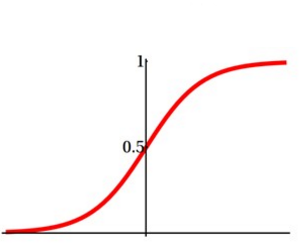
\includegraphics[width=5cm]{Bilder/Umsetzung/Sigmoid.PNG}}
\hfill
\subfigure[Tanh]{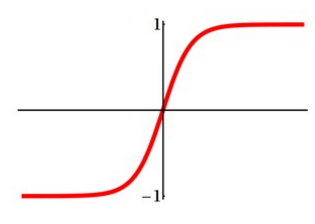
\includegraphics[width=5cm]{Bilder/Umsetzung/tanh.PNG}}
\hfill
\caption{Die Sigmoide Funktion und die Tanh Funktion im Vergleich}
\label{fig:sigtanh}
\end{figure}

\begin{equation}\formelentry{Sigmoide Funktion sowie Tanh Funktion}
(a)\ f(x)= \frac{1}{1+e^{-cx}}\ \ \ \ \ \ \ \ \ \ \ (b)\ f(x)= tanh(x)
\end{equation}


Aus der Tabelle \ref{tab:TRANSMSE} können die Ergebnisse dieses Optimierungsschrittes entnommen werden.


\begin{table}[H]
  \centering
  \begin{tabular}{|c|c|c|}
  \hline 
  \rule[0ex]{0pt}{2.5ex} Transferfunktion & Training-MSE & Test-MSE \\ 
  \hline 
  \rule[0ex]{0pt}{2.5ex} \textbf{Sigmoid} & $9.406 \cdot 10^{-4}$ & $0.001767$\\ 
  \hline 
  \rule[0ex]{0pt}{2.5ex} Tanh & $0.0103333$ & $0.044330$ \\ 
  \hline 
  \end{tabular} 
  \caption{Jeweilige Transferfunktionen \& korrespondierende MSE}
  \label{tab:TRANSMSE}
\end{table}

Man erkennt, dass es sich bei der bisher genutzten sigmoiden Funktion bereits um die beste Lösung handelt. Folglich wurde das KNN in dieser Hinsicht nicht weiter optimiert und die ursprüngliche Funktion wurde belassen.

\subsection{Wahl der optimalen Lernregel}
\label{subsection:Wahl der optimalen Lernregel}

Als letzten Schritt wurde die Lernregel des KNN optimiert. Innerhalb des Verfahrens der überwachten Lernens existieren mehrere Lernregeln, um das Netz zu trainieren. Die bekannteste Lernregel ist die Backpropagation-Lernregel. Diese Regel gibt es in mehreren Variationen. In dieser Seminararbeit werden zum einen das Grundverfahren sowie einige Variationen, namentlich das  "`Momentum Backpropagation"' sowie das "`Resilient Backpropagation"' beschrieben und untersucht. Anschließend wird das für die Anwendung am besten geeignete Verfahren ausgewählt\footnote{\Vgl\Zitat{Laemmel}, S. 225 f.}.

\begin{itemize}
\item \textbf{Backpropagation}:\\
Dies ist das klassische Fehlerrückführungsverfahren zum Anpassen der Verbindungsgewichte. Die Gewichtsveränderung erfolgt durch ein Fehlersignal, dass aus der Abweichung von tatsächlicher und prognostizierter Ausgabe berechnet wird. Die Gewichtsveränderung erfolgt hierbei schichtweise von den Ausgangs-Neuronen bis zu den Eingangs-Neuronen.

\item \textbf{Momentum Backpropagation}:\\
Dieses Verfahren fügt dem klassischen Verfahren einen Trägheitsterm hinzu, indem die Gewichtsveränderung zum Zeitpunkt $t-1$ berücksichtigt wird. Dieser Term kann einen Wert zwischen $0$ und $1$ annehmen. Umso größer dieser Term ist, umso stärker wir die vorhergehende Gewichtsveränderung berücksichtigt. Durch diesen Trägheitsterm wird die Wahrscheinlichkeit verringert, dass das KNN beim Training in ein lokales Minimum oszilliert und sich somit nicht weiter dem Idealwert approximieren kann. Auch die Wahl der Lernrate gestaltet sich hier weniger kritisch. 

\item \textbf{Resilient Propagation}:\\
Resilient heißt Federnd. Dieses Verfahren nutzt das Vorzeichen das Gradienten zum Zeitpunkt $t$ und entscheidet anhand dessen, ob das Gewicht vergrößert oder verkleinert werden muss. Der Betrag der Gewichtsveränderung wird jedoch unabhängig von der Richtung der Gewichtsänderung ermittelt.  Dadurch werden die typischen Probleme klassischer Gradientenabstiegsverfahren, wie sie beim klassischen Backpropagation sowie beim Momentum Backpropagation genutzt werden, gemindert.\footnote{\Vgl\Zitat{Valen}, S. 71}.

Die Formeln für Resilient Propagation lauten wie folgt:

\begin{equation}\formelentry{Formel zur Bestimmung der Art der Gewichtsänderung}
\Delta w_{ij}=\begin{cases} 
-\Delta_{ij} & falls S(t) > 0 \\ 
+\Delta_{ij} & falls S(t) < 0  \\ 
\pm 0       & sonst 
\end{cases}
\end{equation}

\begin{equation}\formelentry{Formel zur Bestimmung des Betrages der Gewichtsänderung}
\Delta_{ij}=\begin{cases} 
\Delta_{ij}(t-1)\cdot n^+ & falls S(t-1) \cdot S(t) > 0 \\ 
\Delta_{ij}(t-1)\cdot n^- & falls S(t-1) \cdot S(t) < 0 \\
\Delta_{ij}(t-1)       & sonst 
\end{cases}
\end{equation}


Solange das Vorzeichen des Gradienten negativ ist, wird das Vorzeichen des Gewichtes ebenfalls beibehalten und die Schrittweite und somit das Gewicht um einen konstanten Wert $n^{+}$ vergrößert. Somit können Plateaus besser überwunden werden.
Ändert sich das Vorzeichen des Gradienten von negativ auf positiv(was bedeutet, dass ein Minimum übersprungen wurde), so wird das Vorzeichen geändert und die Schrittweite um  einen fixen Faktor $n^{-}$ verringert. Somit werden Oszillationen verhindert.

Die Abbildung \ref{fig:RP} stellt das Vorgehen des Resilient Propagation Algorithmus grafisch dar\footnote{\Vgl\Zitat{Geith}, S. 71}.

\begin{figure}[H]
	\centering
	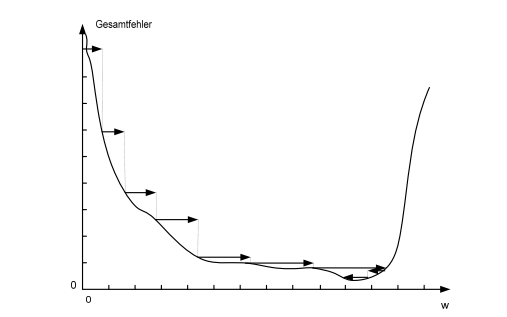
\includegraphics[width=10cm]{Bilder/Umsetzung/VisuResi.PNG}
	\caption{Visualisierung des Resilient Propagation Algorithmus}
	\label{fig:RP}
\end{figure}

\end{itemize}

Allen drei Lernregeln ist gemein, dass zur Bestimmung des Fehlers zwischen der prognostizierten und tatsächlichen Ausgabe der MSE benutzt werden kann. Die MSE-Formel würde in dem konkreten Fall der Anwendung wie folgt lauten:

\begin{equation}\formelentry{MSE zur Berechnung der Abweichung}
   \frac{1}{2}\sum^{n}_{i=1} (KT_{i} - KV_{i})^2
\end{equation}

Wobei $n$ für die Anzahl der Daten im Datensatz steht, $KT_i$ für den tatsächlichen Ausgabewert eines Datum $i$ steht und $KV_i$ für den korrespondierenden prognostizierten Ausgabewert eines Datums $i$ steht.

In der Tabelle \ref{tab:LERNregeln} kann das Ergebnis der Trainings- und Testdurchläufe mit den jeweiligen Lernregeln betrachtet werden.

\begin{table}[H]
  \centering
  \begin{tabular}{|c|c|c|}
  \hline 
  \rule[0ex]{0pt}{2.5ex} Lernregel & Training-MSE & Test-MSE \\ 
  \hline 
  \rule[0ex]{0pt}{2.5ex} Backpropagation & $9.325\cdot10^{-4}$ & $0.001636$ \\ 
  \hline 
  \rule[0ex]{0pt}{2.5ex} Momentum Backpropagation & $9.109\cdot10^{-4}$ & $0.001608$ \\ 
  \hline 
  \rule[0ex]{0pt}{2.5ex} \textbf{Resilient Propagation} & $8.89\cdot10^{-4}$ & $9.406\cdot10^{-4}$ \\ 
  \hline 
  \end{tabular} 
  \caption{Lernregeln \& jeweilige MSE}
  \label{tab:LERNregeln}
\end{table}

In der Regel liefert Resilient Propagation sehr gute Ergebnisse, dies ist auch hier der Fall. Wie man erkennen kann, ist das Resilient Propagation Verfahren  hier den anderen überlegen. Folglich wurde das KNN entsprechend optimiert und Resilient Propagation als Lernregel eingesetzt. Da es sich bei Resilient Propagation um eine adaptive Lernregel handelt und bei der Berechnung keine Lernrate benutzt handelt, muss diese auch nicht angegeben werden.

\section{Die endgültigen künstlichen neuronalen Netze}
\label{section:Die endgültigen künstlichen neuronalen Netze}

Nachdem das KNN zur Prognose des DAX erstellt und optimiert wurde, wurden diese Schritte in analoger weise für die KNN zur Prognose des Nikkei sowie zur Prognose des Dow Jones wiederholt.
Es stellte sich heraus, dass das optimale KNN für den DAX ebenfalls das Optimale KNN für den Nikkei und den Dow Jones darstellt. Das Endgültige Netz sowie dessen Parameter können aus der Tabelle \ref{tab:ENDconf} sowie aus der  Abbildung \ref{fig:ENDKNN} entnommen werden.

\begin{table}[H]
  \centering
  \begin{tabular}{|c|c|}
  \hline 
  \rule[0ex]{0pt}{2.5ex}  Topologie & 4-7-1 mit Bias\\ 
  \hline 
  \rule[0ex]{0pt}{2.5ex}  Lernregel & Resilient Propagation\\  
  \hline 
  \end{tabular} 
  \caption{Die jeweiligen Börsenkurse \& deren Endwerte}
  \label{tab:ENDconf}
\end{table}

\begin{figure}[H]
	\centering
	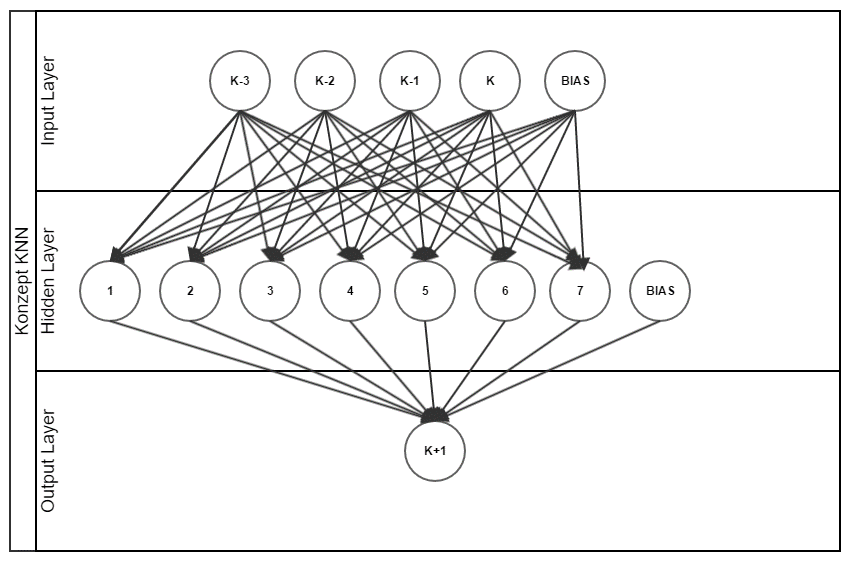
\includegraphics[width=10cm]{Bilder/Umsetzung/FertigKNN.PNG}
	\caption{Das endgültige KNN für alle Börsenkurse}
	\label{fig:ENDKNN}
\end{figure}

Die Tabelle \ref{tab:ENDval} zeigt die Trainings- sowie Testergebnisse der implementierten und optimierten KNN nach jeweils $200.000$ Trainingszyklen.

\begin{table}[H]
  \centering
  \begin{tabular}{|c|c|c|}
  \hline 
  \rule[0ex]{0pt}{2.5ex}  Börsenkurs & Training-MSE & Test-MSE\\ 
  \hline 
  \rule[0ex]{0pt}{2.5ex} DAX & $4.252\cdot10^{-5}$ & $4.820\cdot10^{-5}$  \\ 
  \hline 
  \rule[0ex]{0pt}{2.5ex} Nikkei & $1.350\cdot10^{-5}$ & $4.520\cdot10^{-5}$  \\ 
  \hline 
   \rule[0ex]{0pt}{2.5ex} Dow Jones & $6.672\cdot10^{-5}$ & $2.820\cdot10^{-4}$  \\ 
  \hline 
  \end{tabular} 
  \caption{Die endgültigen Parameter für alle KNN}
  \label{tab:ENDval}
\end{table}
